\chapter{需求建模}
\section{数据流图}
\subsection{顶层数据流图}
\subsection{0层数据流图}
\begin{figure}[H]
\centering
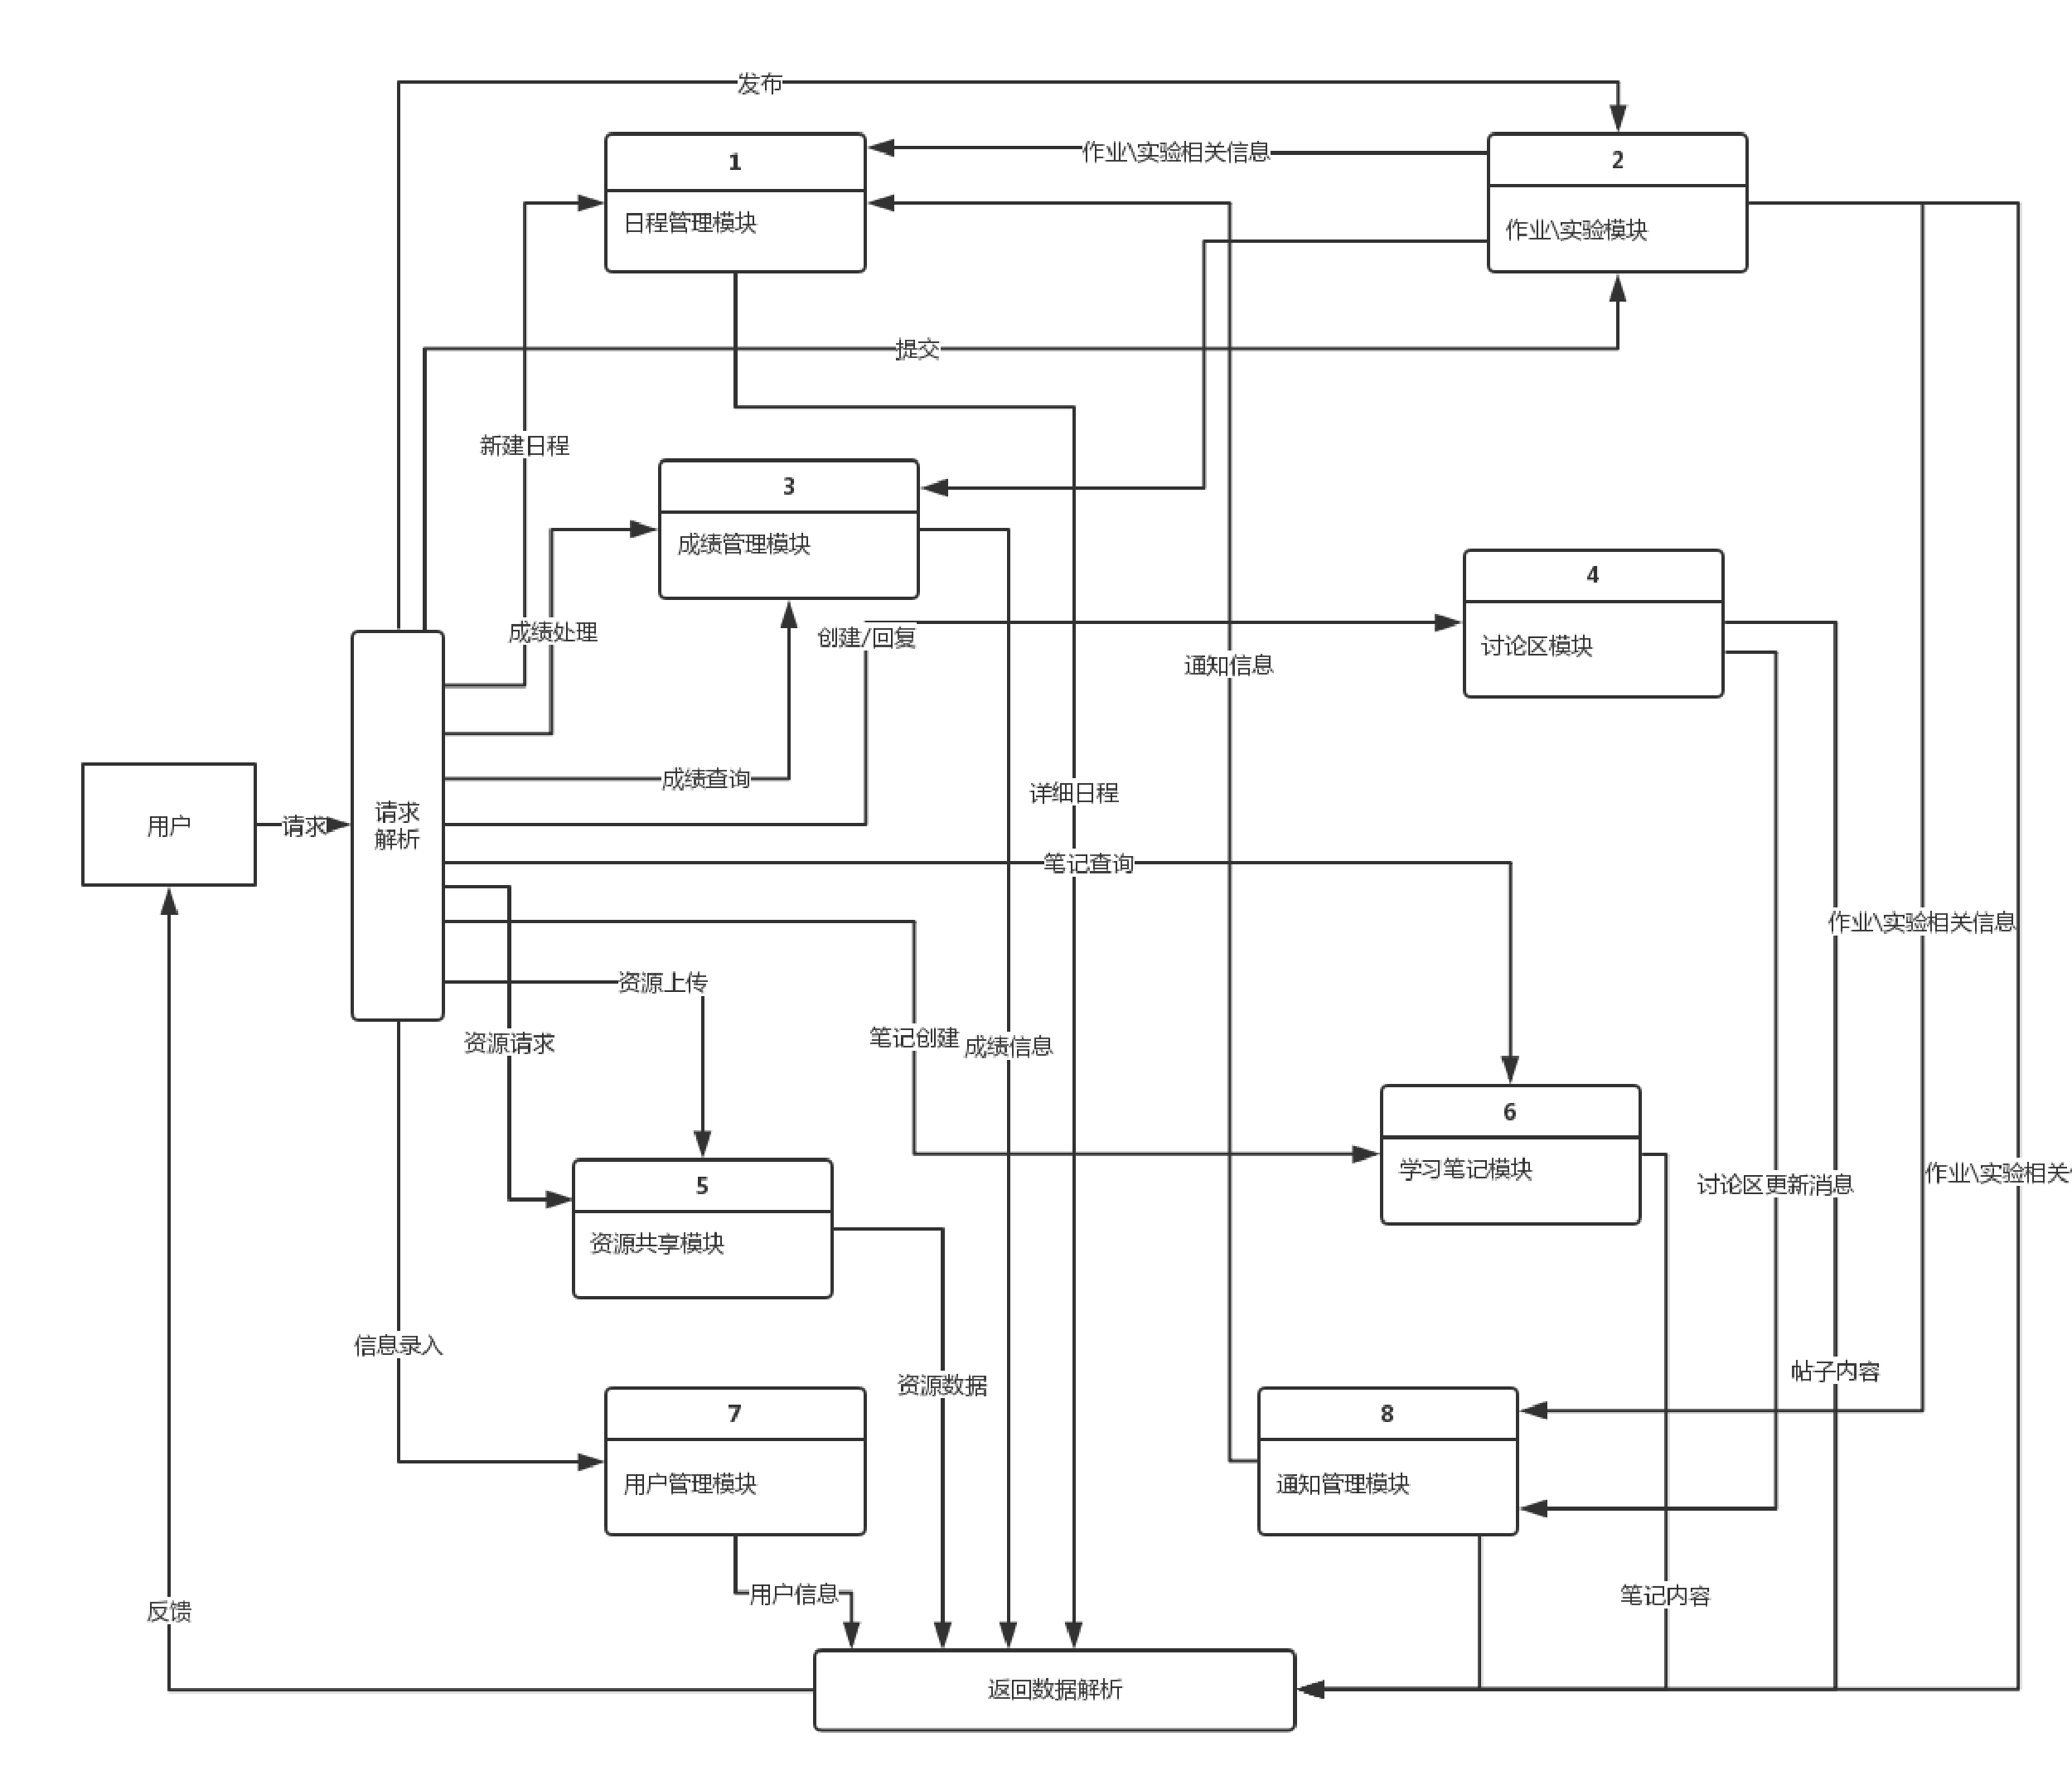
\includegraphics[width=15cm]{Level_0}
\caption{0层数据流图}
\end{figure}
\subsection{1层数据流图}
\subsubsection{日程管理模块}
\begin{figure}[H]
\centering
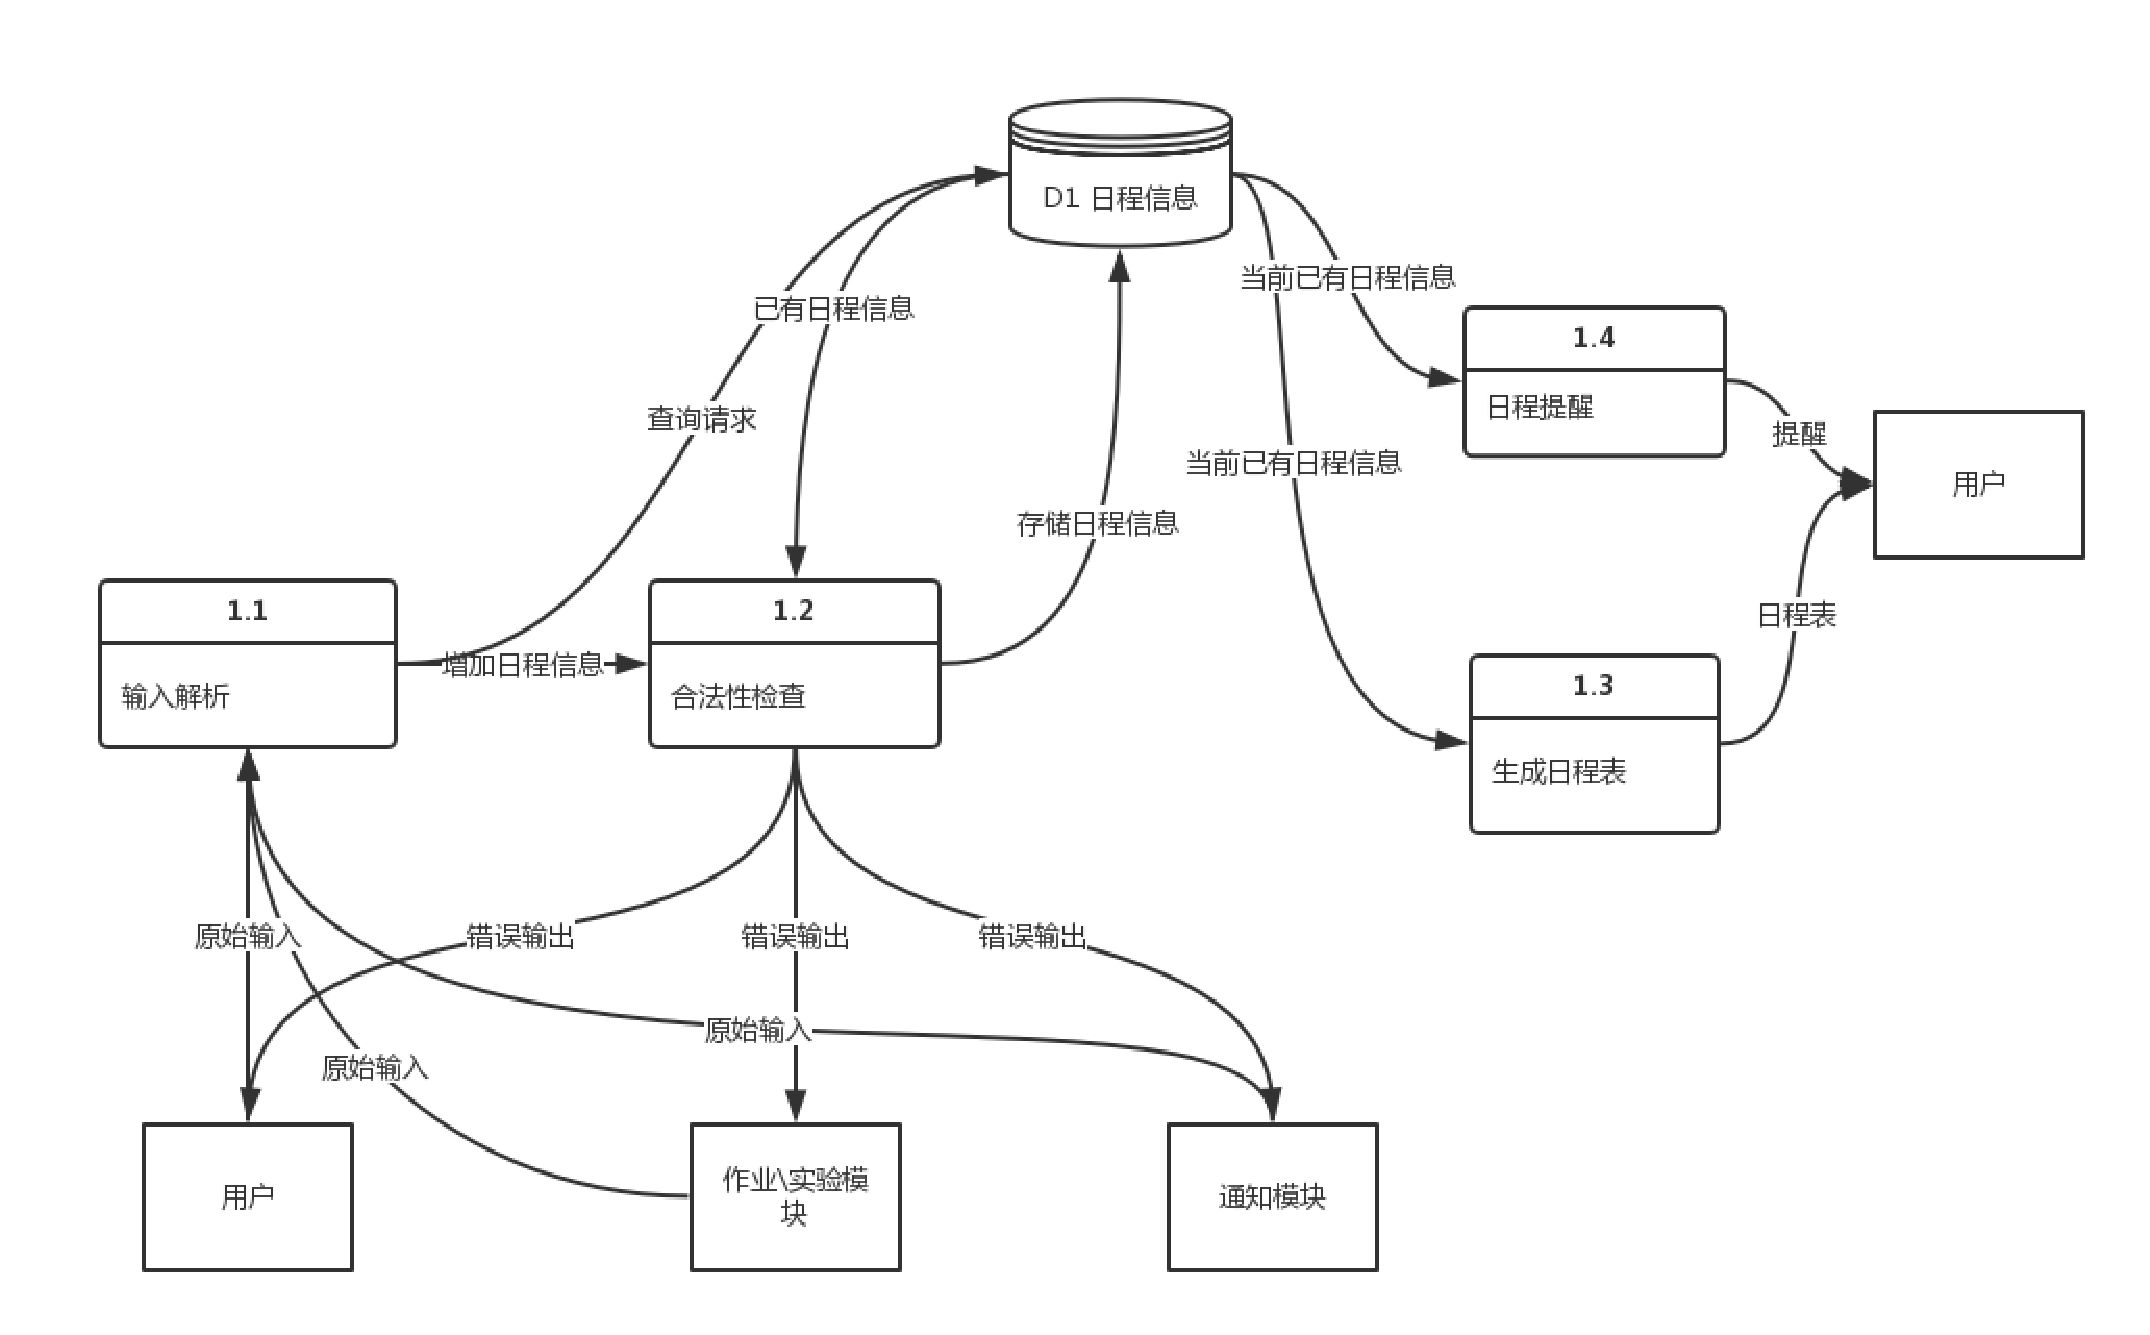
\includegraphics[width=15cm]{level1_1}
\caption{日程管理模块功能数据流图}
\end{figure}
\subsubsection{作业实验模块}
\begin{figure}[H]
\centering
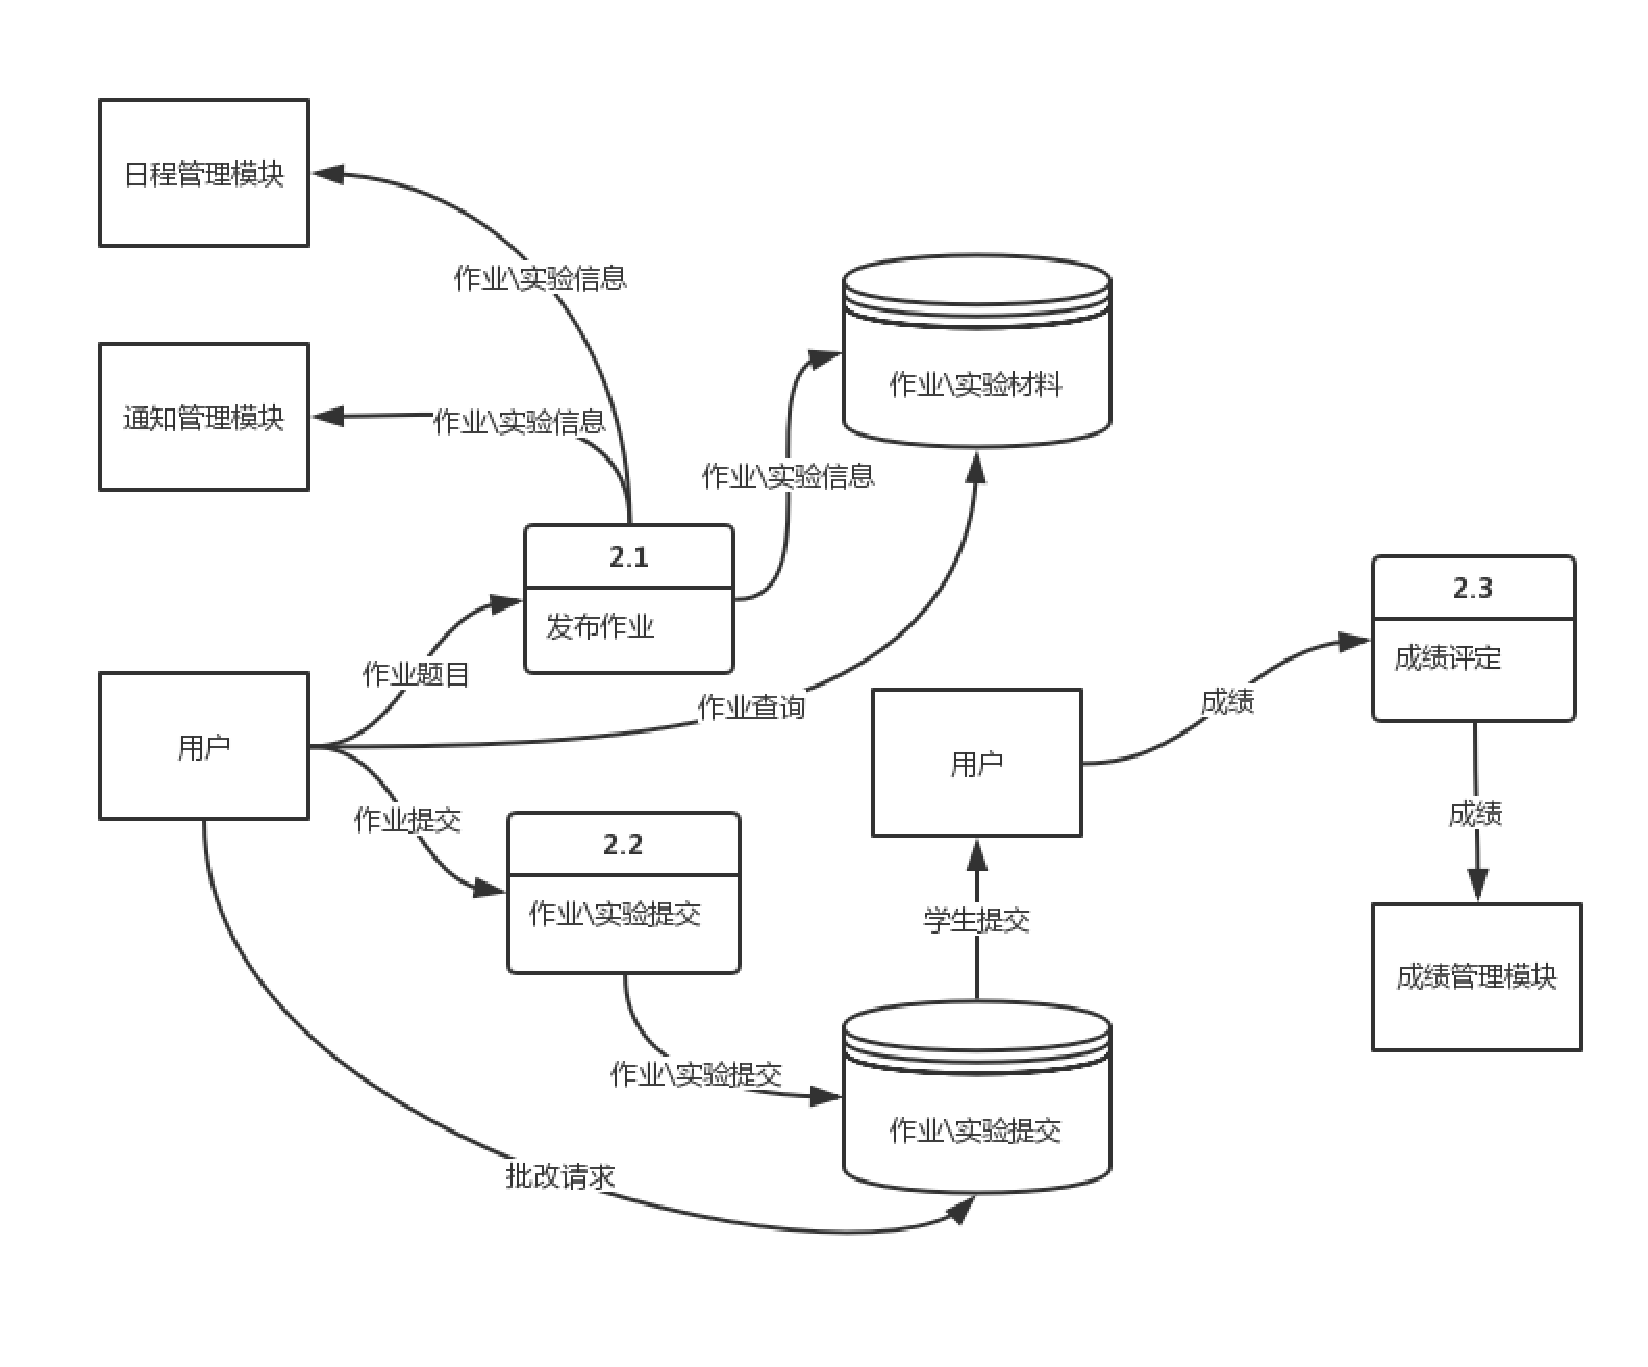
\includegraphics[width=15cm]{level1_2}
\caption{日程管理模块功能数据流图}
\end{figure}
\subsubsection{学习笔记模块}
\begin{figure}[H]
\centering
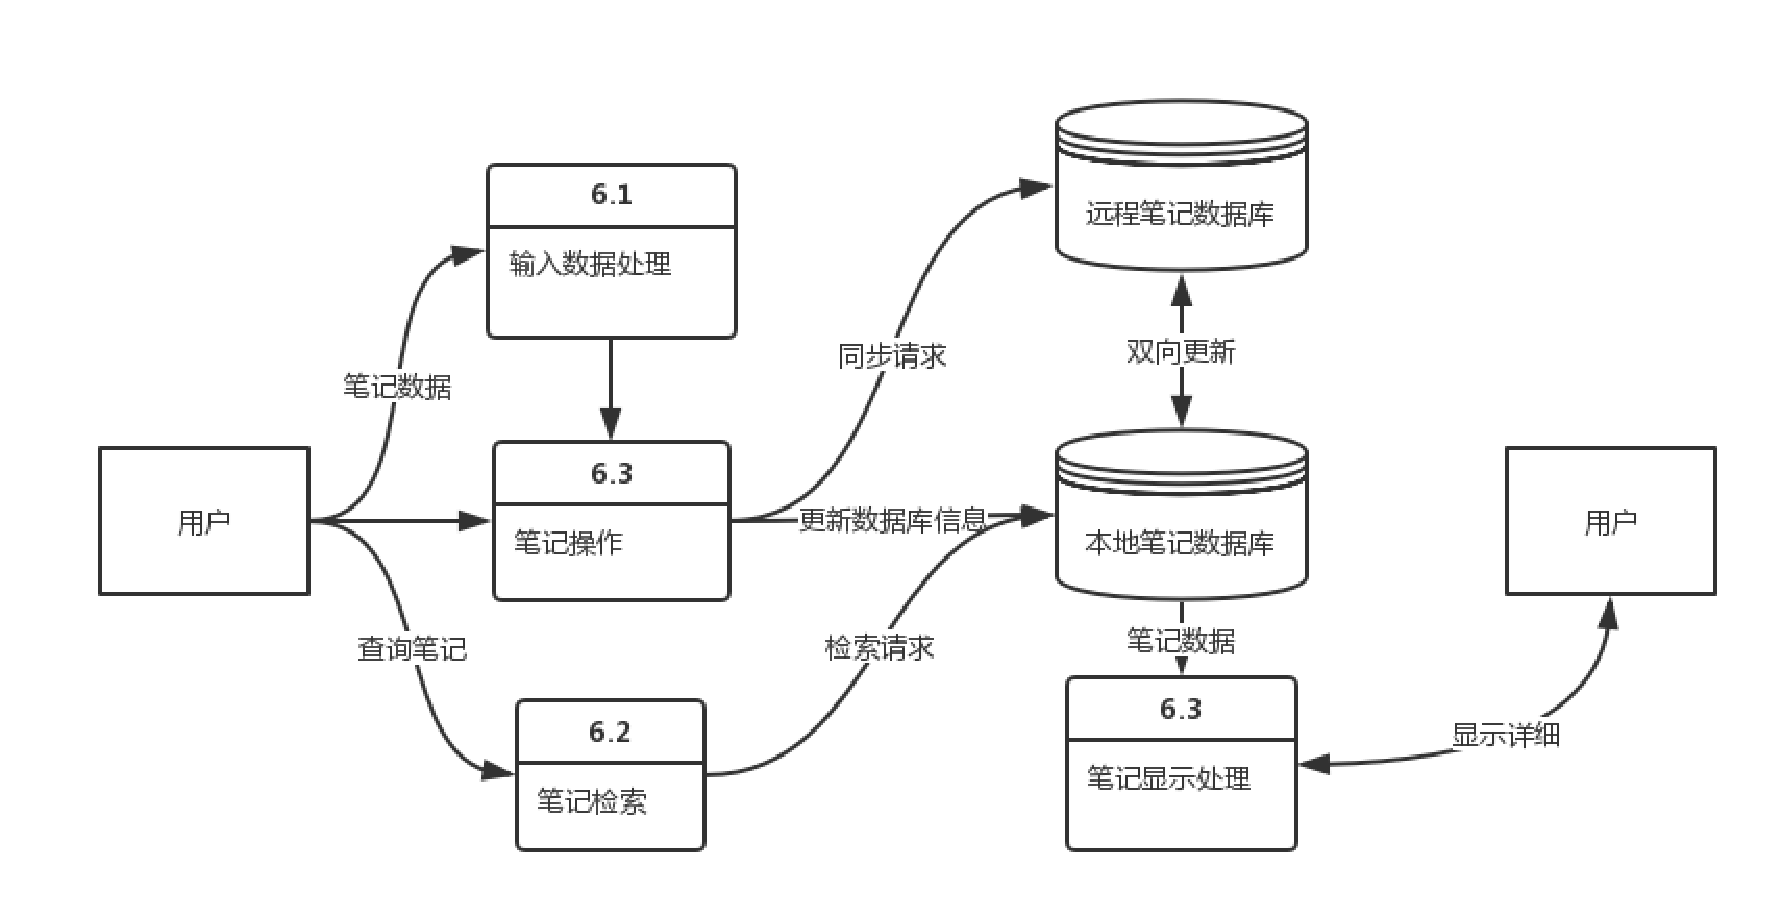
\includegraphics[width=15cm]{level1_3}
\caption{学习笔记模块功能数据流图}
\end{figure}
\subsubsection{成绩管理模块}
\begin{figure}[H]
\centering
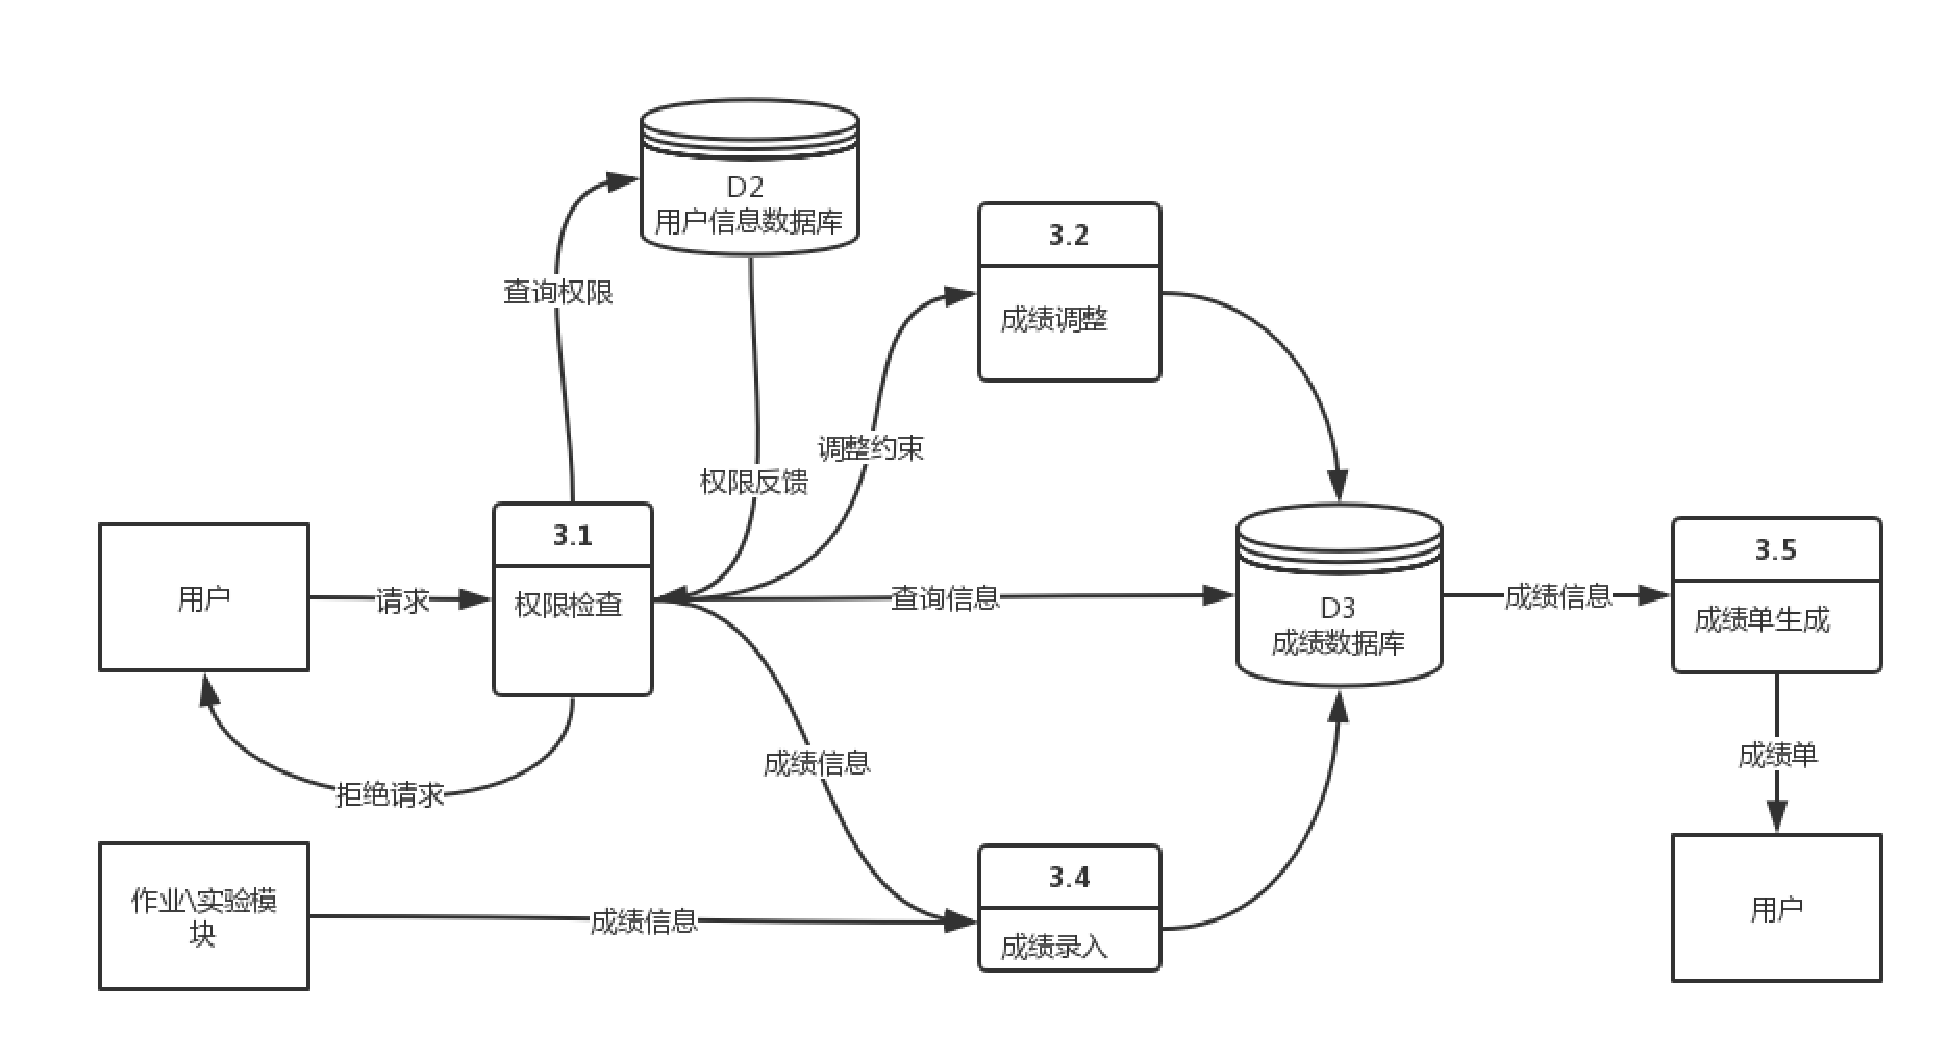
\includegraphics[width=15cm]{level1_4}
\caption{成绩管理模块功能数据流图}
\end{figure}
\subsubsection{用户管理模块}
\begin{figure}[H]
\centering
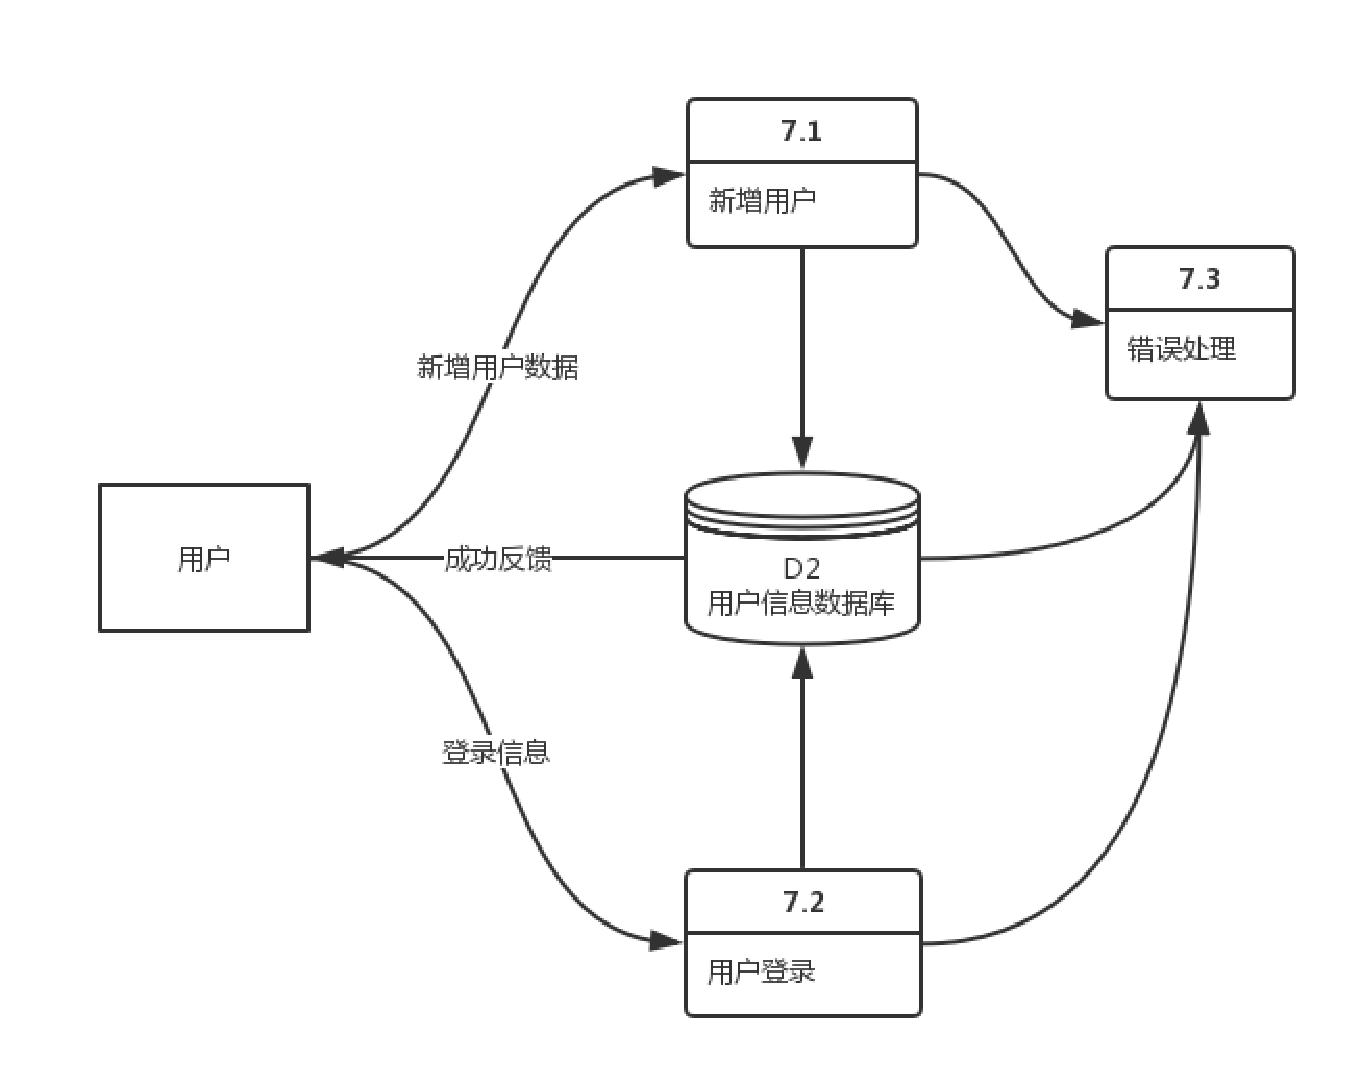
\includegraphics[width=15cm]{level1_5}
\caption{用户理模块功能数据流图}
\end{figure}
\subsubsection{讨论区模块}
\begin{figure}[H]
\centering
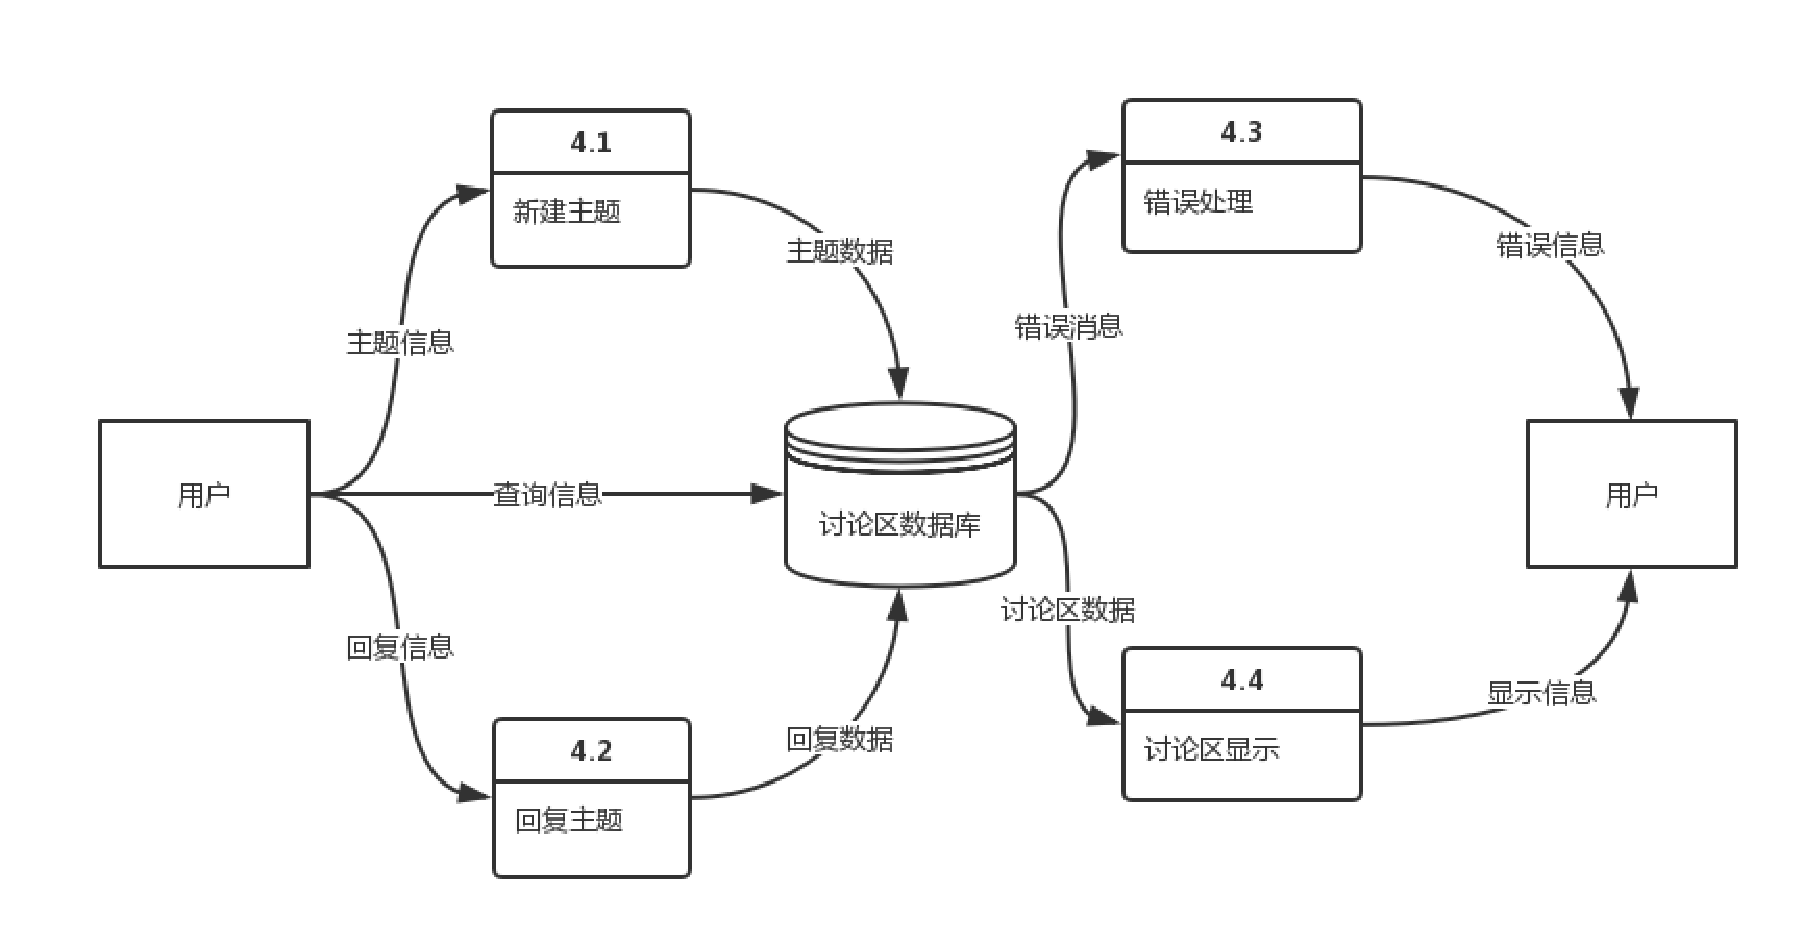
\includegraphics[width=15cm]{level1_6}
\caption{讨论区模块功能数据流图}
\end{figure}
\subsubsection{资源共享模块}
\begin{figure}[H]
\centering
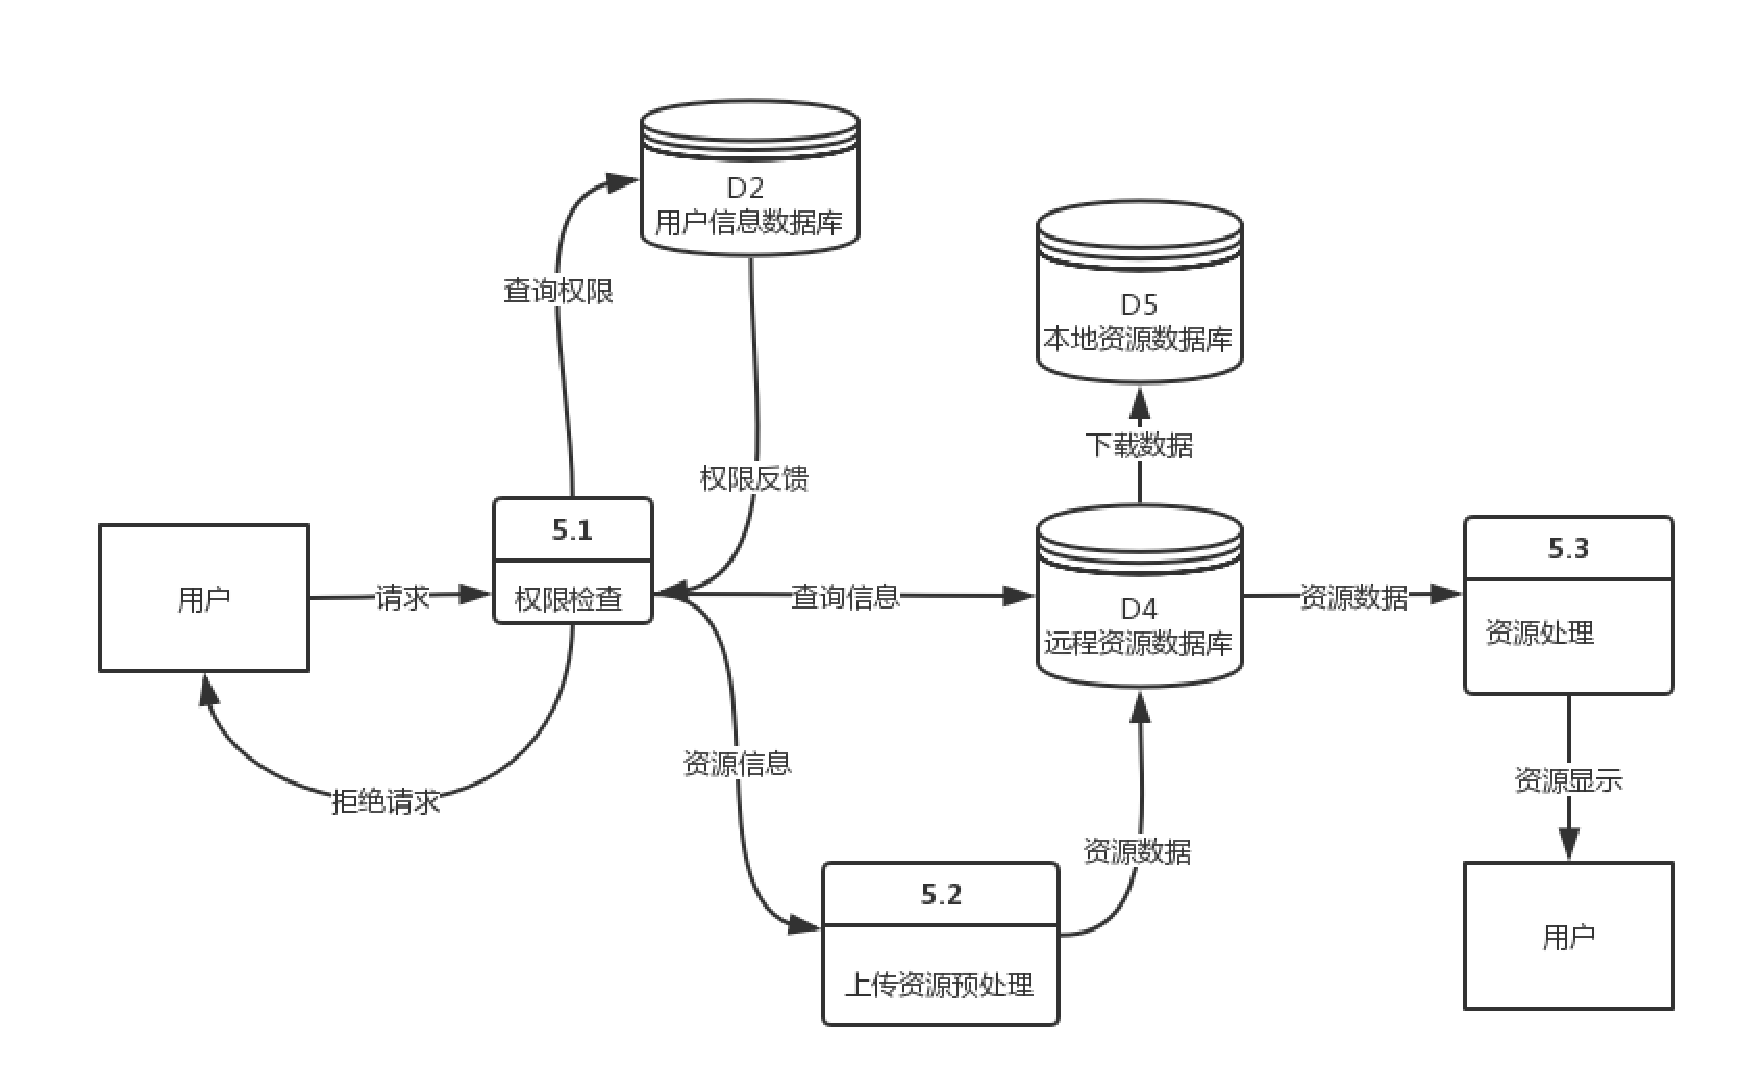
\includegraphics[width=15cm]{level1_7}
\caption{资源共享模块功能数据流图}
\end{figure}
\subsubsection{通知管理模块}
\begin{figure}[H]
\centering
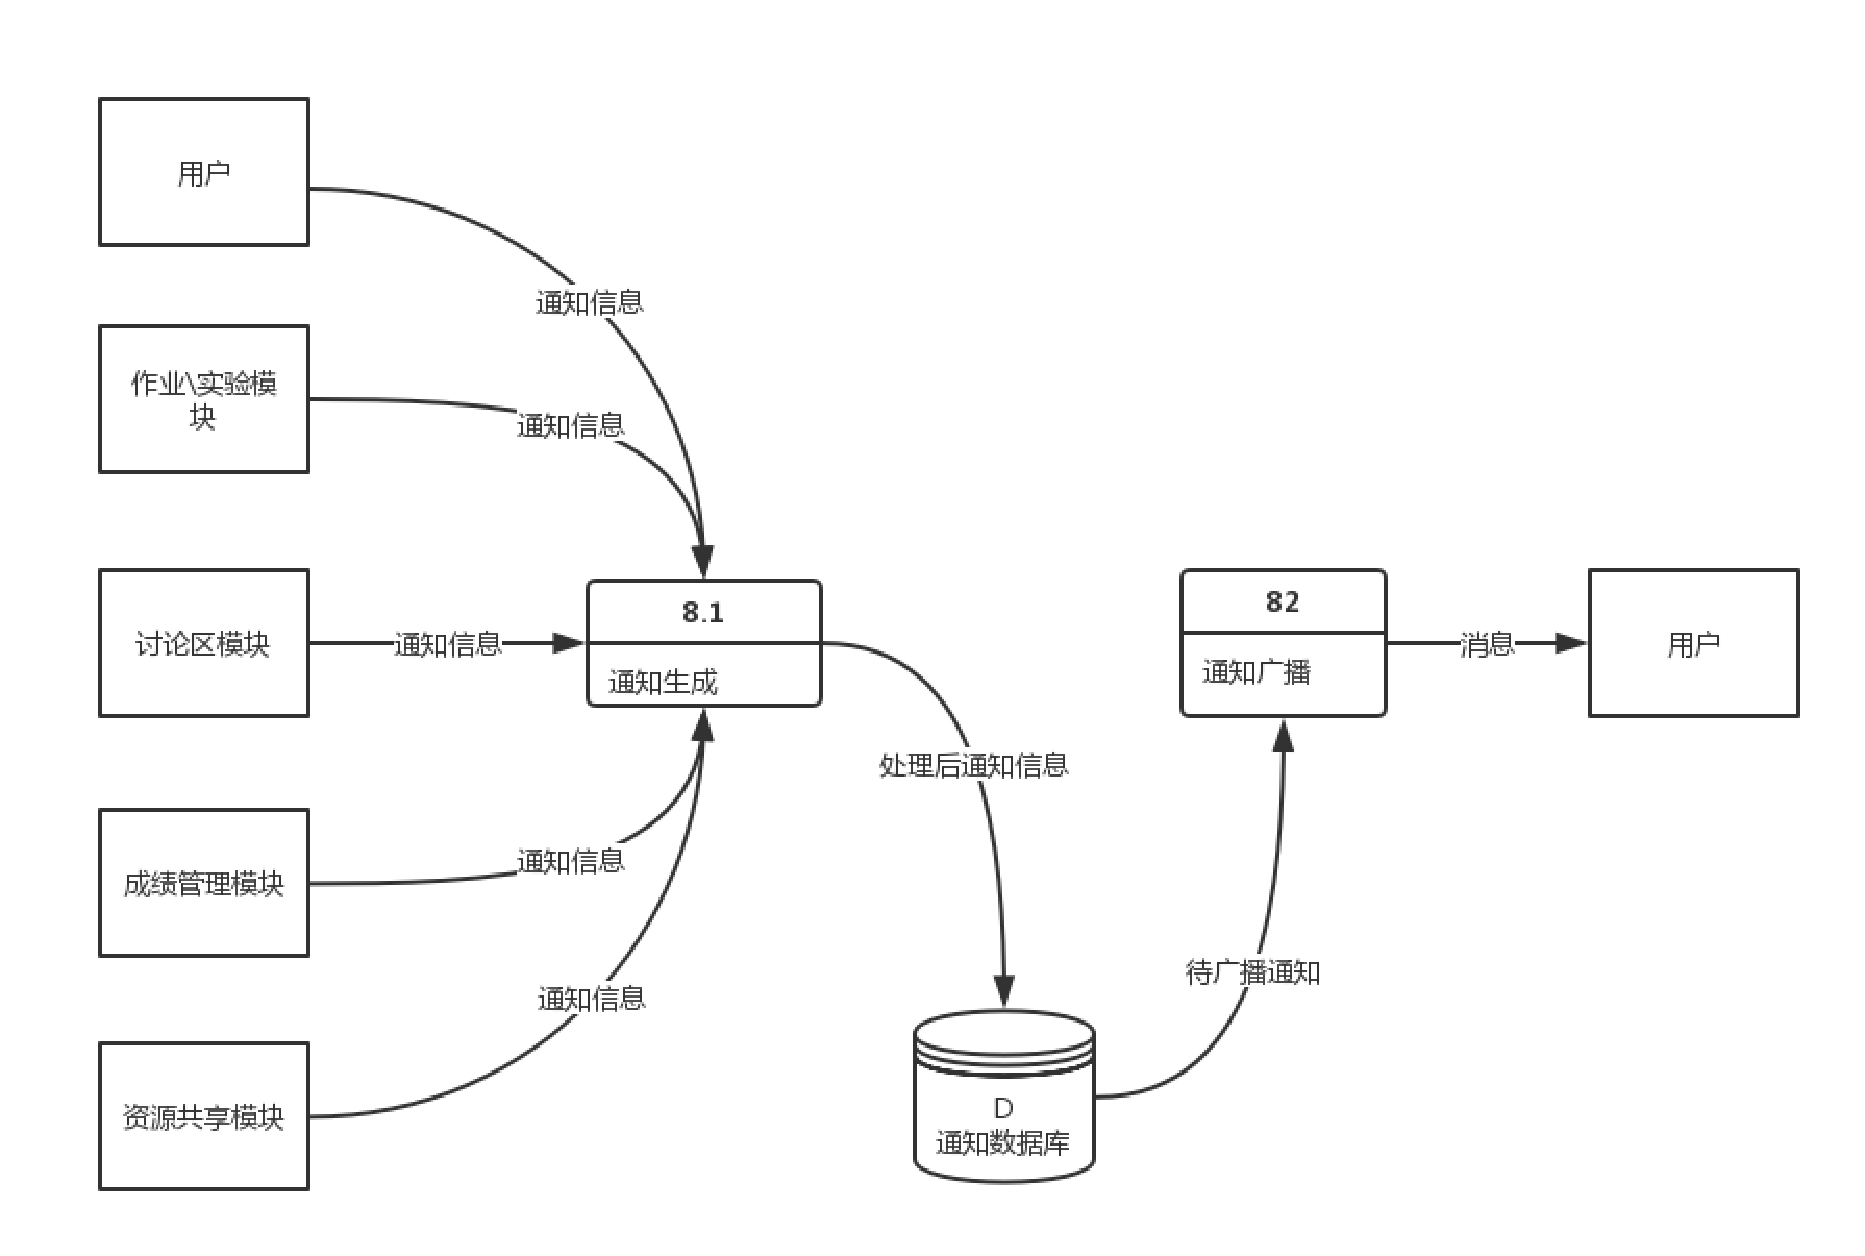
\includegraphics[width=15cm]{level1_8}
\caption{通知管理模块功能数据流图}
\end{figure}

\section{数据字典}
\subsection{数据流说明}
\subsubsection{请求}
\begin{description}
  \item[来源]用户
  \item[简述]用户对数据“请求操作”
  \item[去向]请求解析
\end{description}

\subsubsection{信息录入}
\begin{description}
  \item[来源]请求解析
  \item[简介]讲用户信息录入数据库
  \item[去向]用户管理模块
\end{description}

\subsubsection{用户信息}
\begin{description}
  \item[来源]用户管理模块
  \item[简介]从数据库中导出的用户信息
  \item[去向]返回数据解析
\end{description}

\subsubsection{反馈}
\begin{description}
  \item[来源]返回数据解析
  \item[简介]客户端对于用户数据的处理结果
  \item[去向]用户
\end{description}

\subsubsection{作业/实验/通知查询}
\begin{description}
  \item[来源]用户
  \item[简介]对作业/实验进行查询请求
  \item[去向]作业/实验材料,日程管理模块,通知模块
\end{description}

\subsubsection{作业/实验/通知发布}
\begin{description}
  \item[来源]用户
  \item[简介]新的作业/实验创建
  \item[去向]发布作业
\end{description}

\subsubsection{作业/实验/通知提交}
\begin{description}
  \item[来源]用户
  \item[简介]提交作业
  \item[去向]作业/实验提交
\end{description}

\subsubsection{作业/实验查看与批改}
\begin{description}
  \item[来源]请求解析
  \item[简介]查看学生提交的作业
  \item[去向]用户,本地数据库
\end{description}

\subsubsection{笔记创建}
\begin{description}
  \item[来源]请求解析
  \item[简介]新的笔记条目的创建
  \item[去向]学习笔记模块
\end{description}


\subsubsection{笔记内容}
\begin{description}
  \item[来源]学习笔记模块
\item[简介]用户查询的笔记内容
\item[去向]返回数据解析
\end{description}




\subsubsection{笔记数据}
\begin{description}
  \item[来源]用户,本地笔记数据库
\item[简介]用户的笔记内容
\item[去向]输入数据处理,笔记操作,笔记显示处理
\end{description}


\subsubsection{查询笔记}
\begin{description}
  \item[来源]用户
\item[简介]对笔记数据进行查询请求
\item[去向]笔记检索
\end{description}

\subsubsection{同步请求}
\begin{description}
  \item[来源]笔记操作
\item[简述]客户端与远程笔记同步
\item[去向]远程笔记数据库
\end{description}

\subsubsection{更新数据库信息}
\begin{description}
  \item[来源]笔记操作
\item[简述]向客户端提出更新数据库命令
\item[去向]本地笔记数据库
\end{description}


\subsubsection{双向更新}
\begin{description}
  \item[来源]远程笔记数据库,本地笔记数据库
\item[简述]客户端与远程笔记双向更新
\item[去向]远程笔记数据库,本地笔记数据库
\end{description}

\subsubsection{检索请求}
\begin{description}
  \item[来源]笔记检索
\item[简述]在客户端查询笔记
\item[去向]本地笔记数据库
\end{description}

\subsubsection{显示详细}
\begin{description}
  \item[来源]笔记显示处理
\item[简述]将笔记数据显示到用户界面
\item[去向]用户
\end{description}

\subsubsection{新增用户数据}
\begin{description}
  \item[来源]用户
\item[简介]在数据库中增加用户
\item[去向]新增用户
\end{description}

\subsubsection{成功反馈}
\begin{description}
  \item[来源]用户信息数据库
\item[简介]反馈给用户新增数据成功
\item[去向]用户
\end{description}

\subsubsection{登录信息}
\begin{description}
  \item[来源]用户,用户登录
\item[简介]将用户的登录信息在用户和客户端间同步
\item[去向]用户,用户登录
\end{description}

\subsubsection{主体信息}
\begin{description}
  \item[来源] 用户
  \item[简介] 新建主题以及简单描述
  \item[去向] 新建主题
\end{description}

\subsubsection{查询信息}
\begin{description}
  \item[来源] 用户
  \item[简介] 查询显示讨论区的相关信息
  \item[去向] 讨论区数据库
\end{description}

\subsubsection{回复信息}
\begin{description}
  \item[来源] 用户
  \item[简介] 回复内容
  \item[去向] 回复主题
\end{description}

\subsubsection{资源请求}
\begin{description}
  \item[来源] 用户
  \item[简介] 用户请求获取相关资源
  \item[去向] 权限检查
\end{description}

\subsubsection{查询权限}
\begin{description}
  \item[来源] 权限检查
  \item[简介] 检查用户的请求是否具有相应的执行权限
  \item[去向] 用户信息数据库
\end{description}




\subsection{数据存储说明}
\subsubsection{讨论区数据库}
\begin{description}
  \item[简述] 存储讨论区相关内容信息
  \item[数据排列] 降温被内容单独存储。同时以关键词等建立索引。并且另外建表存储创建者日期权限等信息
\end{description}

\subsubsection{本地资源数据库}
\begin{description}
  \item[简述] 存储用户下载和导入的本地资源数据
  \item[数据排列] 根据用户系统平台选用相应文件系统的存储方式。同时依据用户的选择建立权限等数据库表单
\end{description}
\subsubsection{远程资源数据库}
\begin{description}
  \item[简述] 存储用户服务器端的数据
  \item[数据排列] 分布式存储,尽量减少重复信息的存储。同时依据用户的选择建立权限等数据库表单
\end{description}
\subsubsection{日程信息数据库}
\begin{description}
  \item[简述] 存储用户日程相关信息
  \item[数据排列] 根据用户,日期,描述等键值建表
\end{description}
\subsubsection{成绩数据库}
\begin{description}
  \item[简述] 存储用户成绩相关信息
  \item[数据排列] 根据用户、成绩以及何次作业或者考试建表
\end{description}
\subsubsection{数据库发布作业/实验/通知存储}
\begin{description}
  \item[简述] 服务器数据库存放教师发布的作业/实验/通知
  \item[数据排列] 数据存在多个lable,主要的主键有发布课程编号,类型,作业号。其列名还有内容,截至日期,附件地址等。
\end{description}

\subsubsection{作业附件存储}
\begin{description}
  \item[简述] 服务器存放教师发布的作业/实验材料
  \item[数据排列] 不同的科目有不同的文件夹,存放到相应的文件夹下。将地址存入数据库相应的部分。
\end{description}

\subsubsection{学生提交作业/实验存储}
\begin{description}
  \item[简述] 服务器存放学生上传的作业/实验。
  \item[数据排列]数据库的主键为作业号。其列名还有学生学号,名称,作业/实验提交与否,地址。
  将学生提交的内容存入服务器的文件夹下,地址放入上述服务器。若使用git提交,则同样保存按照git服务器保存在服务器上。
\end{description}

\subsubsection{用户账号数据库存储}
\begin{description}
  \item[简述]服务器端数据库存储用户的邮箱,学号,姓名,密码,用户权限,选修课程,课程详情等基本信息
  \item[数据排列]数据存在多个table,以用户邮箱,学生姓名,课程名称为主键,数据按主键排列
\end{description}

\subsubsection{笔记数据库存储}
\begin{description}
\item[简述]存储在服务器数据库中的用户信息,笔记内容,笔记创建时间,相关学科等信息
\item[数据排列]数据存在多个table,数据以用户账户,笔记学科为主键,笔记按主键排列。
\end{description}

\subsubsection{笔记数据库本地存储}
\begin{description}
\item[简述] 存储在客户端数据库中的笔记内容,笔记创建时间,相关学科等信息
\item[数据排列] 数据存在多个table,数据以笔记创建时间,笔记学科为主键,笔记按主键排列。
\end{description}






\subsection{加工说明}
\subsubsection{新建主题}
检查用户提供信息是否合法。然后将其中的图片公式等等转换格式存入数据库中。
\subsubsection{回复信息}
检查用户回复是否合法。然后将其中的图片公式等等转换格式存入数据库中。
\subsubsection{讨论区显示}
从数据库中获取相关信息,处理渲染之后发送给用户客户端显示。
\subsubsection{权限检查}
根据用户请求从数据库中获取相关数据并判断是否具有执行操作的权限。
\subsubsection{上传资源预处理}
首先检查上传数据是否有效合法。不合法或者失效给出警告。合法则计算MD5查询数据库中是否已经存在相同资源,存在则只建立相应的链接,不存在则上传文件至远程数据库。
\subsubsection{资源处理}
从远程获取数据,根据数据格式以及用户平台进行相应的转码处理最后交付客户端直接进行显示。
\subsubsection{输入解析}
日程的输入有多种格式,如果用户输入的不是标准的各项信息,而是纯文本等等,则首先尝试从中解析出事件地点描述等关键信息,尝试构建日程,成功则存入数据库,失败返回报错。
\subsubsection{日程提醒}
检索当前日程数据库中的相关信息,比较当前日期,如果有满足提醒条件的则给用户发送提醒。
\subsubsection{成绩录入}
根据用户或者其他模块的输入构造满足后台数据存储结构的信息并且存储。
\subsubsection{成绩调整}
解析用户的调整需求看是否合法,如果合法则对数据库进行更新。

\subsubsection{发布作业/实验/通知}
用户将作业/实验/通知填写好发送。

服务器判断用户发来的数据,将附件存入相应空间,将其他内容存入数据库中。

向客户端发送成功与否的信息。

\subsubsection{学生提交作业/实验}
学生将作业/实验内容从本地提交。

服务器接受消息,更新数据库,并将收到的文件存储。

向客户端发送结果信息。

\subsubsection{处理登录}
客户端发送查询请求到服务器用户数据库,匹配该用户邮箱或学号和密码,匹配成功则返回成功登录的信息,并同步数据。匹配失败则返回失败信息,并显示账户不存在或密码错误。

\subsubsection{处理新用户请求}
客户端发送新建请求到服务器数据库,检查是否为新用户,若可创建则返回允许创建信息,失败则返回无法创建新用户。

\subsubsection{处理笔记}
对笔记请求数据处理,分发给下一级功能区具体处理

\subsubsection{创建笔记}
创建新的笔记,创建成功则将新的笔记按用户选择存入本地存储,或存入服务器。

\subsubsection{删除笔记}
删除云端或者本地存储的笔记,返回操作结果。

\subsubsection{处理查询}
从本地存储和服务器存储的的数据文件进行搜索,对于符合关键字的搜索返回给用户,如果没有结果则显示无结果。
